\chapter{RESULTS}
\label{chapter:results}

\section{The Bean 2 prototype Implementation}
The Bean 2 prototype was designed on United Microelectronics Corporation (UMC) RFMM180 technology and send to fabricate through Europractice IC mini@sic program. 
%Special care has been taken to mitigate the effects of electrical and process-related nonidealities, . Common centroid layout, dummy devices and 

Fig.~\ref{fig:IC_layout} shows the layout of the Bean 2 prototype, for a detailed description of the IC pinout, see Apprendix A.



\begin{figure}[!t]
	\centering
	\includegraphics[width=6in]{./Figures/IC_layout}
	\caption{The Bean 2 prototype layout.}\label{fig:IC_layout}
\end{figure}

\begin{figure}[!p]
	\centering
	\includegraphics[width=4in]{./Figures/CSA_layout}
	\caption{Charge-sensitive amplifier layout.}\label{fig:csa_layout}
\end{figure}

\begin{figure}[!t]
	\centering
	\includegraphics[width=4.5in]{./Figures/OTA_layout}
	\caption{Recycling folded cascode OTA layout.}\label{fig:ota_layout}
\end{figure}

\begin{figure}[!t]
	\centering
	\includegraphics[width=4.5in]{./Figures/buffer_layout}
	\caption{Rail-to-rail operational amplifier layout.}\label{fig:buffer_layout}
\end{figure}

\begin{figure}[!t]
	\centering
	\includegraphics[width=6in]{./Figures/filter_layout}
	\caption{Filter Layout.}\label{fig:filter layout}
\end{figure}



\section{Filter simulation results}


\begin{figure}[!t]
	\centering
	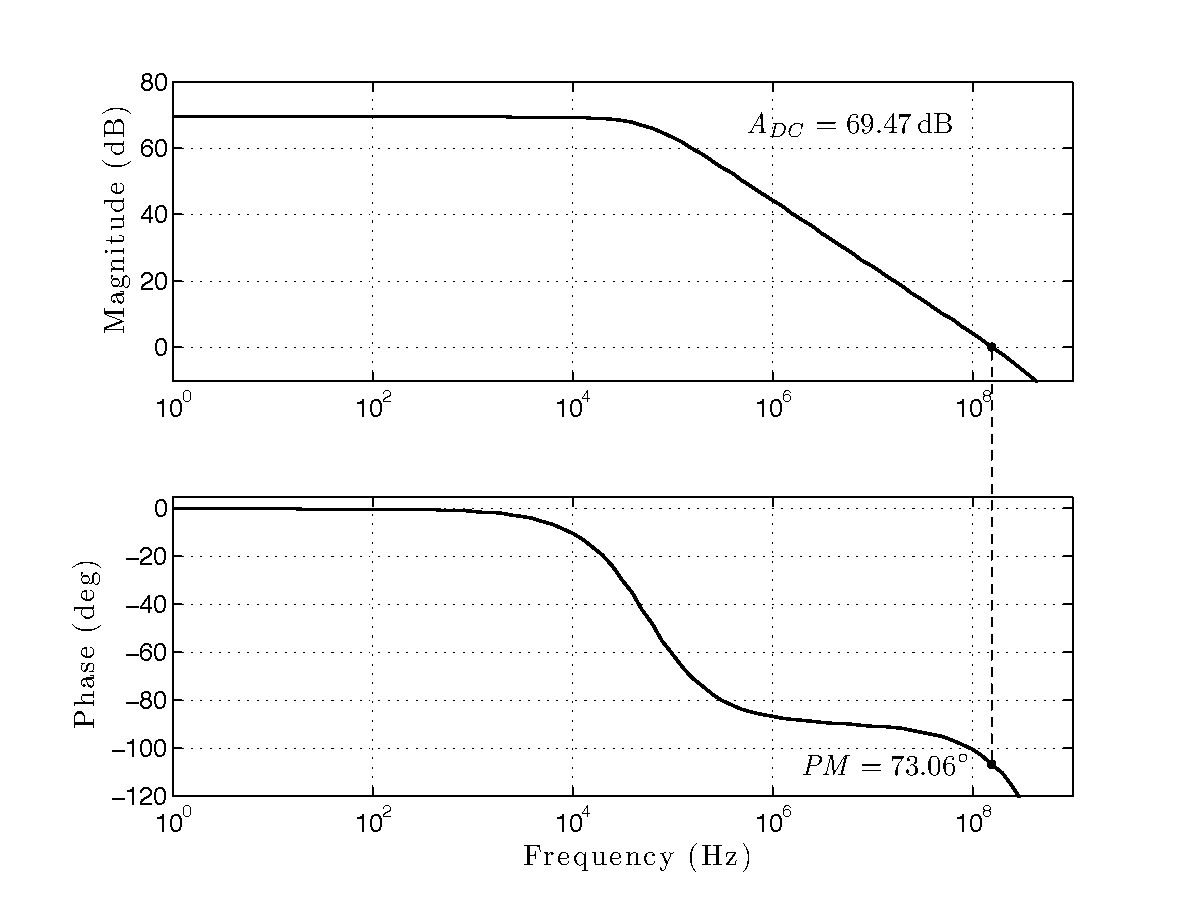
\includegraphics[width=5.3in]{./Test/bode_OTA_post}
	\caption{Bode plot for the OTA open-loop response.}\label{fig:bode_OTA}
\end{figure}

\begin{figure}[!t]
	\centering
	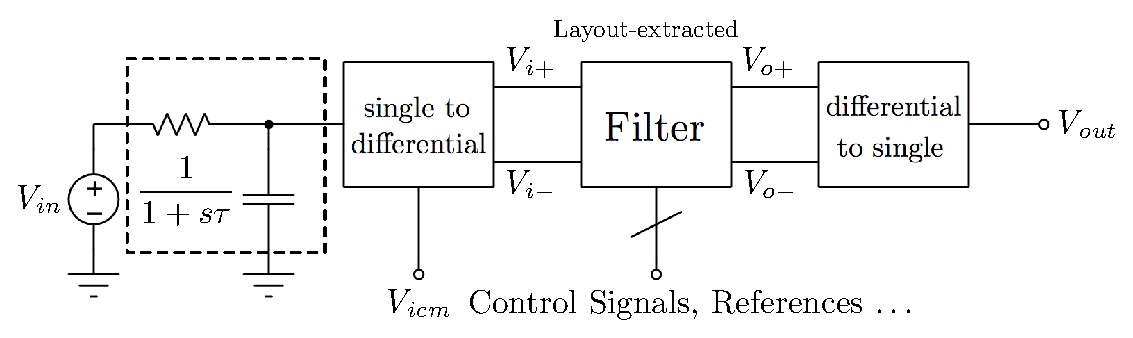
\includegraphics[width=5in]{./Test/wf_test_circuit}
	\caption{Weighting function test circuit.}\label{fig:wf_test_circuit}
\end{figure}

\begin{figure}[!t]
	\centering
	\includegraphics[width=3.6in]{./Test/sim_wf}
	\caption{SPICE-simulated weighting function. $\tau=8\,\text{ns}$, $N=16$ and $T_s=19.25\,\text{ns}$.}\label{fig:sim_wf}
\end{figure}


\begin{figure}[!t]
	\centering
	\includegraphics[width=4.4in]{./Test/gain_curves.pdf}
	\caption{Filter output step response with the 64 programmable gains. \mbox{$V_\textit{in}=0.1\,V$} and \mbox{$T_s=40\,\text{ns}$}.}\label{fig:gain_curves}
\end{figure}

\begin{figure}[!t]
	\centering
	\includegraphics[width=4.4in]{./Test/linearity.pdf}
	\caption{Filter linearity test results, full-scale input range.}\label{fig:gain_curves}
\end{figure}

\begin{figure}[!t]
	\centering
	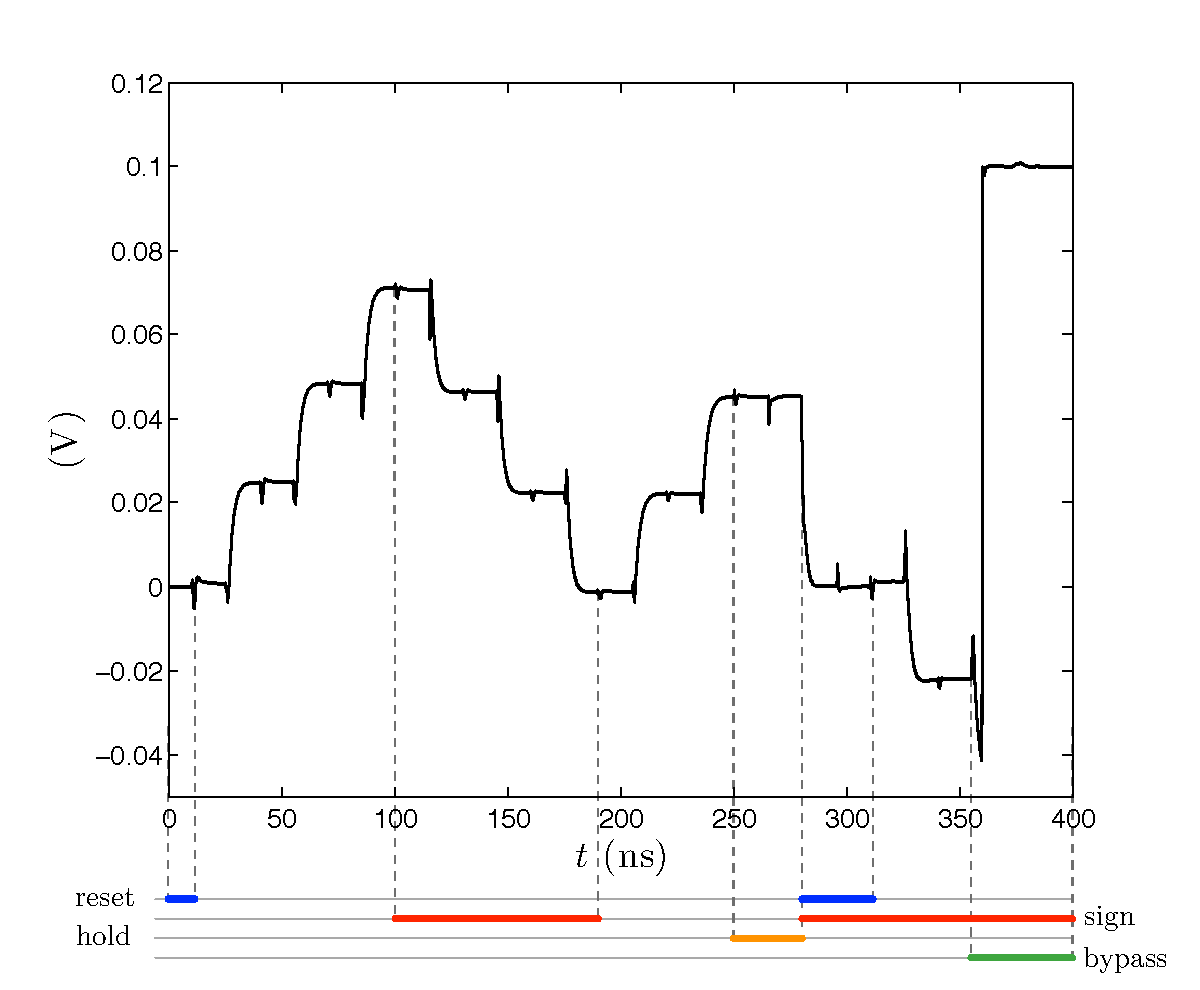
\includegraphics[width=5in]{./Test/test_filter_after_omni.eps}
	\caption{Filter control signals testing. $V_\textit{in}=0.1\,V$ and $\text{gain}=0.25\,V/V$.}\label{fig:test_filter_after_omni}
\end{figure}

\begin{figure}[!t]
	\centering
	\includegraphics[width=5.3in]{./Test/bode_buffer_post}
	\caption{Bode plot for the buffer open-loop response.}\label{fig:bode_buffer}
\end{figure}